\documentclass[a4j]{ujarticle}
\usepackage[dvipdfmx]{graphicx}
\usepackage{url}
\usepackage{bbding}
\usepackage{lscape}
\usepackage[subrefformat=parens]{subcaption}
\usepackage{bm}
\usepackage{amsmath}

\title{進捗報告資料}
\author{安達智哉\\to-adachi@ist.osaka-u.ac.jp}
\date{2019年5月29日}

\begin{document}
\maketitle


\section{メモリ負荷の算出}
文献\cite{3gpp.23.720}に示されているコネクション確立に伴うシグナリング図を図\ref{Legacy_connection_setup}に示す。
UEがIdle状態からConnected状態へ遷移する際に各ノードのメモリが保持する情報についてOAIのソースコード(OpenairinterfaceCN-develop)を元に調査を行っている。
具体的には、各シグナリングを処理する際に各ノードがメモリに格納する情報をリストアップし、それらの情報量を足し合わせることによりメモリ負荷を推定する。
今回は、MMEが関与している以下のシグナリングを処理する際にMMEが保持する情報を調査した。
\begin{itemize}
  \item S1-AP Initial UE msg
  \item S1-AP Initial Ctxt Setup Request
  \item S1-AP Initital Ctxt Setup Compl
  \item Modify Bearer Request
  \item Modify Bearer Response
  \item S1-AP UE Ctxt Release Req
  \item Release Access Bearers Req
  \item Release Access Bearers Resp
  \item S1-AP UE Ctxt Release Cmd
  \item S1-AP UE Ctxt Release Compl
\end{itemize}
\begin{figure}[htbp]
  \centering
  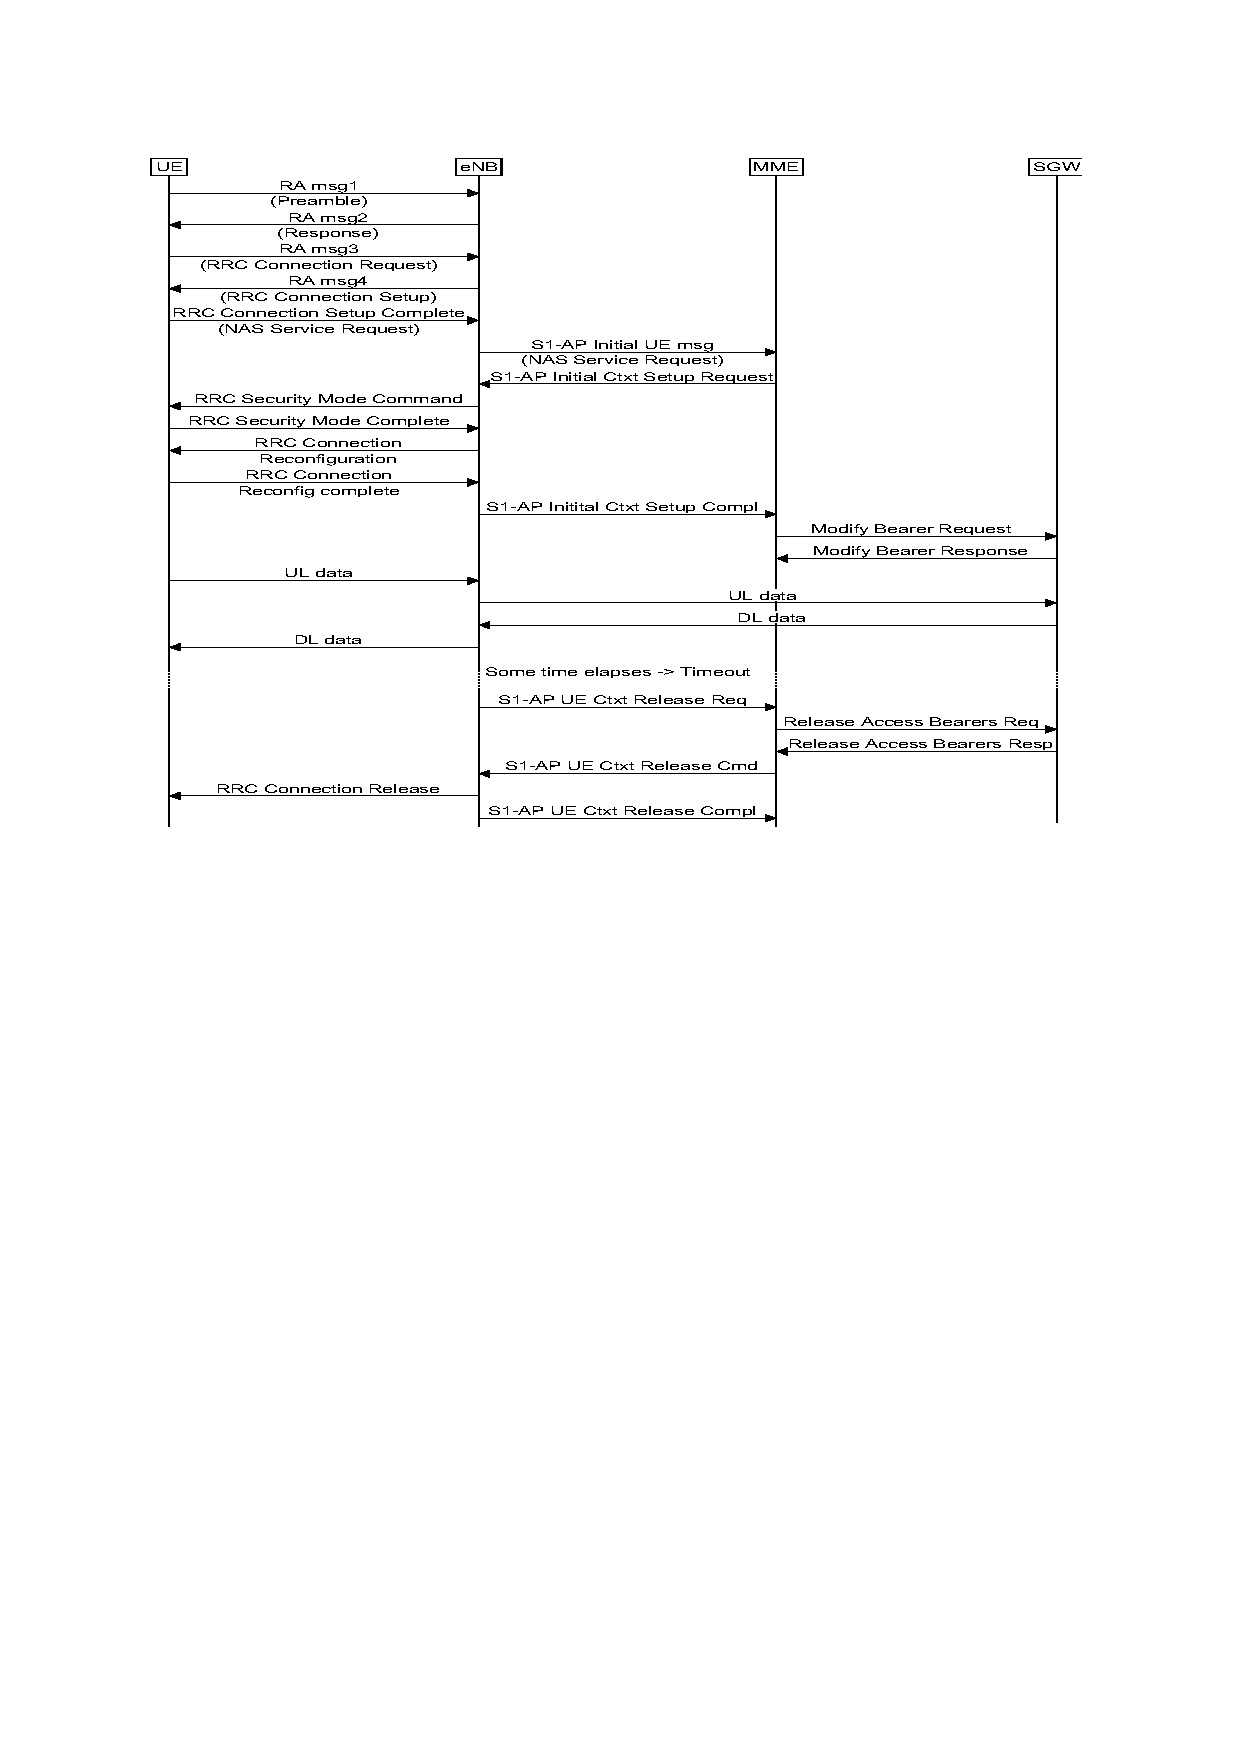
\includegraphics[width=0.9\hsize]{Legacy_connection_setup.pdf}
  \caption{Legacy connection setup}
  \label{Legacy_connection_setup}
\end{figure}

\clearpage
MMEは各シグナリングを受信、送信する際に保持する情報を以下の表\ref{table:oai_source_memory}に示す。

S1-AP Initial UE msgを受信した際は、約2KBの分の構造体を生成しており、この構造体にUEのコンテキストやベアラ情報を格納している。
S1-AP Initital Ctxt Setup Complの受信とModify Bearer Requestの送信処理では、メモリに情報を追加する処理は行っていない。。
Modify Bearer Responseを受信した際は、MMEの持つUEのステートに関する情報の更新を行っている。しかし、メモリに保持する情報量に変化はない。


S1-AP UE Ctxt Release Reqを受信した際は、MMEが保持しているUEのステートをConnectedからIdleへ変更する処理や次のシグナリングであるRelease Access Bearers Reqの準備等を行っているが、メモリに保持する情報の追加や削除は行われていない。
Release Access Bearers Reqの送信の処理処理ではメモリ操作はない。
Release Access Bearers Respを受信してからS1-AP UE Ctxt Release Cmdを送信するまでの処理で、MMEの管理するベアラ情報の更新を行う。
S1-AP UE Ctxt Release Complを受信した際に UEのコンテキストを削除している。


\begin{table}[htbp]
  \centering
  \caption{シグナリングメッセージを処理する際にMMEが保持する情報}
  \label{table:oai_source_memory}
  \begin{tabular}{l|l|c}
    \hline
    シグナリング  & 情報名 & 情報量(bit)  \\ \hline \hline
    S1-AP Initial UE msg & \verb|ue_description_s| & 408 \\
    & \verb|ue_context_s| & 17470\\\hline
    S1-AP Initital Ctxt Setup Compl & - & 0 \\\hline
    Modify Bearer Request & - & 0 \\\hline
    Modify Bearer Response & - & 0 \\\hline
    S1-AP UE Ctxt Release Req & - & 0 \\\hline
    Release Access Bearers Req & - & 0 \\\hline
    Release Access Bearers Resp & - & 0 \\\hline
    S1-AP UE Ctxt Release Compl & \verb|ue_context_s| & -17470 \\\hline

  \end{tabular}
\end{table}

S1-AP Initial UE msgを処理する際にMMEは、\verb|ue_description_s|という名前の構造体を保持することが表\ref{table:oai_source_memory}より分かる。この構造体の中身を以下の表\ref{table:oai_source_memory_ue_description_s}に示す。
\begin{table}[htbp]
  \centering
  \caption{ue\_description\_sのメンバ}
  \label{table:oai_source_memory_ue_description_s}
  \begin{tabular}{l|l}
    \hline
    メンバ & 情報量(bit) \\ \hline \hline
    \verb|enb_description_s| & 32\\
    \verb|s1_ue_state_s| & 160\\
    \verb|enb_ue_s1ap_id_t|  & 24\\
    \verb|mme_ue_s1ap_id_t| & 32\\
    \verb|sctp_stream_id_t (s ctp_stream_recv)| & 16\\
    \verb|sctp_stream_id_t (s ctp_stream_send)| & 16\\
    \verb|s11_sgw_teid| & 32\\
    \verb|outcome_response_timer_id| & 32\\
    \verb|s1ap_ue_context_rel_timer| & 64\\\hline
    合計  & 408\\\hline
  \end{tabular}
\end{table}

\begin{table}[htbp]
  \centering
  \caption{ue\_context\_sのメンバ}
  \label{table:oai_source_ue_context_s}
  \begin{tabular}{l|l}
    \hline
    メンバ & 情報量(bit) \\ \hline \hline
    \verb|imsi| & 64\\
    \verb|imsi_auth| & 1\\
    \verb|enb_s1ap_id_key_t| & 64\\
    \verb|enb_ue_s1ap_id_t| & 24\\
    \verb|mme_ue_s1ap_id_t | & 32\\
    \verb|sctp_assoc_id_t | & 32\\
    \verb|ue_context_rel_cause| & 224\\ %441
    \verb|subscription_known| & 1\\
    \verb|msisdn[MSISDN_LENGTH+1]| & 128\\
    \verb|msisdn_length| & 8\\
    \verb|mm_state| & 64\\
    \verb|ecm_state| & 64\\
    \verb|is_guti_set| & 8\\
    \verb|guti| & 80\\ %353
    \verb|me_identity| & 240\\
    \verb|e_utran_cgi| & 56\\
    \verb|cell_age| & 64\\
    \verb|access_mode| &128 \\
    \verb|apn_profile| &356 \\
    \verb|access_restriction_data| & 32\\%876
    \verb|sub_status| & 96\\
    \verb|subscribed_ambr| & 128\\
    \verb|used_ambr| & 128\\
    \verb|rau_tau_timer| & 32\\
    \verb|*ue_radio_capabilities| & 8\\
    \verb|ue_radio_cap_length| & 32\\
    \verb|mme_s11_teid| & 32\\
    \verb|sgw_s11_teid| & 32\\
    \verb|paa| & 328\\%816
    \verb|pending_pdn_connectivity_req_imsi[16]| & 128\\
    \verb|pending_pdn_connectivity_req_imsi_length| & 8\\
    \verb|pending_pdn_connectivity_req_apn| & 72\\
    \verb|pending_pdn_connectivity_req_pdn_addr| & 72\\
    \verb|pending_pdn_connectivity_req_pti| & 32\\
    \verb|pending_pdn_connectivity_req_ue_id| & 32\\
    \verb|pending_pdn_connectivity_req_qos| & 160\\
    \verb|pending_pdn_connectivity_req_pco| & 784\\
    \verb|pending_pdn_connectivity_req_request_type| & 32\\
    \verb|default_bearer_id| & 8\\
    \verb|eps_bearers[BEARERS_PER_UE]| & 13464\\
    \verb|mobile_reachability_timer| & 64\\
    \verb|implicit_detach_timer| & 64\\
    \verb|initial_context_setup_rsp_timer| & 64\\\hline%14984
    合計  & 17470\\\hline
  \end{tabular}
\end{table}
\clearpage


\section{eNodeBが追加された時のメモリ負荷}
新規のeNodeBが接続した際には、\verb|enb_description_s|という構造体が生成され、この情報をMMEが保持する。
この構造体の中身を表\ref{table:oai_source_enb_description_s}に示す。
この構造体のサイズは225 bytesであることが分かった。
\begin{table}[htbp]
  \centering
  \caption{enb\_description\_sのメンバ}
  \label{table:oai_source_enb_description_s}
  \begin{tabular}{l|l}
    \hline
    メンバ & 情報量(bit) \\ \hline \hline
    \verb|s1_state| & 128\\
    \verb|enb_name[150]| & 1200\\
    \verb|enb_id| & 32\\
    \verb|default_paging_drx| & 8\\
    \verb|nb_ue_associated| & 32\\ %1400
    \verb|ue_coll| & 320\\
    \verb|sctp_assoc_id| & 32\\
    \verb|next_sctp_stream| & 16\\
    \verb|instreams| & 16\\
    \verb|outstreams| & 16\\ \hline %400
    合計  & 1800\\\hline
  \end{tabular}
\end{table}



\section{考察・今後の課題}
今回の調査結果から、UEがIdle状態とConnected状態それぞれの状態にあるときにMMEのメモリに与える負荷が明らかになった。
今回の結果では、UE 1台がIdle状態である時は、約408 bitのメモリ負荷が発生していると考えられる。
またConnected状態である時は、約17,470 bitのメモリ負荷が発生していると考えられる。

また、eNodeBが新しく追加された時は、約1,800bit のメモリ負荷が発生することも分かった。

ここで以前調査した、上野さんの実験データに基づくMMEのメモリ負荷を図\ref{fig:mme_memory}に示す。
この図では、UE及びeNodeBを増加させつつUEのアタッチ処理を完了した際にどれほどのメモリ負荷がMMEに発生するかを示している。
図の結果では、UE1台のアタッチ処理のために約750 KBのメモリ負荷が発生している。

図\ref{fig:mme_memory}の結果と今回の調査結果は直接比較することはが、2桁ほどずれている点は留意すべきである。
上野さんに確認したところ、図\ref{fig:mme_memory}の結果はMMEを起動しているシステム全体のメモリ消費を見ているということであるため、OAI以外のレイヤーの通信プロトコルの処理負荷も含まれていることが分かった。
図\ref{fig:mme_memory}の結果と今回の調査結果の間で大きなずれがある理由は、他の通信プロトコルの負荷の影響である可能性が高い。
\begin{figure}[htbp]
  \centering
  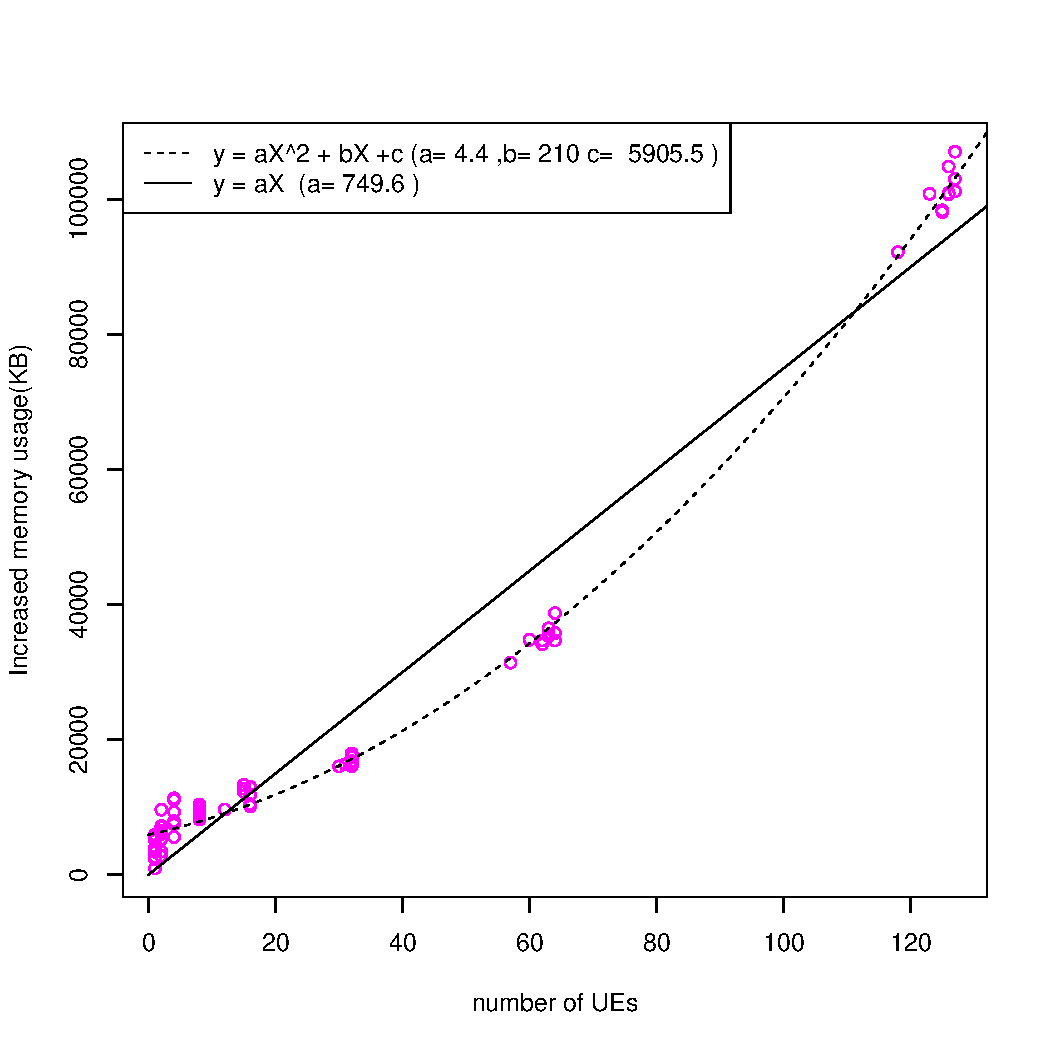
\includegraphics[width=0.9\hsize]{mme_memory.pdf}
  \caption{UE、eNodeBの増加とアタッチ処理の完了によって増加したメモリ負荷(MME)}
  \label{fig:mme_memory}
\end{figure}

  \begin{itemize}
    \item NB-IoT関連の論文を調査する。
    \item 上野さんの実験で発生したパケットを解析する。
    \item Connected Inactive状態において``状態遷移を伴わないデータ送信"が可能なデータ量を調査する。
  \end{itemize}

\section*{\addcontentsline{toc}{section}{参考文献}}
\bibliographystyle{IEEEtran}
\bibliography{/Users/t-adachi/Documents/study/Bibliography/bib/hpt_core_network/myBib/LABbiblio,/Users/t-adachi/Documents/study/Bibliography/bib/hpt_core_network/Study_Group_Bibtex/bib/hptCoreNetwork_Study}
\end{document}
